\documentclass{article}\usepackage[]{graphicx}\usepackage[]{color}
%% maxwidth is the original width if it is less than linewidth
%% otherwise use linewidth (to make sure the graphics do not exceed the margin)
\makeatletter
\def\maxwidth{ %
  \ifdim\Gin@nat@width>\linewidth
    \linewidth
  \else
    \Gin@nat@width
  \fi
}
\makeatother

\definecolor{fgcolor}{rgb}{0.345, 0.345, 0.345}
\newcommand{\hlnum}[1]{\textcolor[rgb]{0.686,0.059,0.569}{#1}}%
\newcommand{\hlstr}[1]{\textcolor[rgb]{0.192,0.494,0.8}{#1}}%
\newcommand{\hlcom}[1]{\textcolor[rgb]{0.678,0.584,0.686}{\textit{#1}}}%
\newcommand{\hlopt}[1]{\textcolor[rgb]{0,0,0}{#1}}%
\newcommand{\hlstd}[1]{\textcolor[rgb]{0.345,0.345,0.345}{#1}}%
\newcommand{\hlkwa}[1]{\textcolor[rgb]{0.161,0.373,0.58}{\textbf{#1}}}%
\newcommand{\hlkwb}[1]{\textcolor[rgb]{0.69,0.353,0.396}{#1}}%
\newcommand{\hlkwc}[1]{\textcolor[rgb]{0.333,0.667,0.333}{#1}}%
\newcommand{\hlkwd}[1]{\textcolor[rgb]{0.737,0.353,0.396}{\textbf{#1}}}%

\usepackage{framed}
\makeatletter
\newenvironment{kframe}{%
 \def\at@end@of@kframe{}%
 \ifinner\ifhmode%
  \def\at@end@of@kframe{\end{minipage}}%
  \begin{minipage}{\columnwidth}%
 \fi\fi%
 \def\FrameCommand##1{\hskip\@totalleftmargin \hskip-\fboxsep
 \colorbox{shadecolor}{##1}\hskip-\fboxsep
     % There is no \\@totalrightmargin, so:
     \hskip-\linewidth \hskip-\@totalleftmargin \hskip\columnwidth}%
 \MakeFramed {\advance\hsize-\width
   \@totalleftmargin\z@ \linewidth\hsize
   \@setminipage}}%
 {\par\unskip\endMakeFramed%
 \at@end@of@kframe}
\makeatother

\definecolor{shadecolor}{rgb}{.97, .97, .97}
\definecolor{messagecolor}{rgb}{0, 0, 0}
\definecolor{warningcolor}{rgb}{1, 0, 1}
\definecolor{errorcolor}{rgb}{1, 0, 0}
\newenvironment{knitrout}{}{} % an empty environment to be redefined in TeX

\usepackage{alltt}
\usepackage{fullpage}
\usepackage[colorlinks=true, linkcolor=blue]{hyperref}
\usepackage{placeins}
\title{Assignment \#1}
\author{Dominic LaRoche}
\IfFileExists{upquote.sty}{\usepackage{upquote}}{}
\begin{document}
\maketitle

I will include embedded code for all analyses in this assignment but please let me know if you would like me to just include one chunk of code at the end of the document.  I first read in the data from the .csv file.\\
\begin{knitrout}
\definecolor{shadecolor}{rgb}{0.969, 0.969, 0.969}\color{fgcolor}\begin{kframe}
\begin{alltt}
\hlkwd{rm}\hlstd{(}\hlkwc{list}\hlstd{=}\hlkwd{ls}\hlstd{())}
\hlstd{crime}\hlkwb{<-}\hlkwd{read.csv}\hlstd{(}\hlstr{"C:/Classes/GeoStat/crime.csv"}\hlstd{)}
\end{alltt}
\end{kframe}
\end{knitrout}

Now we can do some exploration of the variables to see how they are distributed and what the relationships might be between them. Figure \ref{crime} shows the distribution of the crime variable.  We see some depatures from normality, although it is not too severe.  Figure~\ref{hoval} shows the distribtion of the variable ``HOVAL", which has a much more severe depature from normality.  Finally, figure~\ref{inc} gives the sample distribution of the variable ``INC", which also has a strong right skew (similar to ``HOVAL") and does not appear normally distributed.\\
\begin{figure}
\begin{knitrout}
\definecolor{shadecolor}{rgb}{0.969, 0.969, 0.969}\color{fgcolor}\begin{kframe}
\begin{alltt}
\hlkwd{par}\hlstd{(}\hlkwc{mfrow}\hlstd{=}\hlkwd{c}\hlstd{(}\hlnum{1}\hlstd{,}\hlnum{2}\hlstd{))}
\hlkwd{hist}\hlstd{(crime}\hlopt{$}\hlstd{CRIME,}\hlkwc{breaks}\hlstd{=}\hlstr{"Scott"}\hlstd{)}
\hlkwd{qqnorm}\hlstd{(crime}\hlopt{$}\hlstd{CRIME)}
\hlkwd{qqline}\hlstd{(crime}\hlopt{$}\hlstd{CRIME)}
\end{alltt}
\end{kframe}
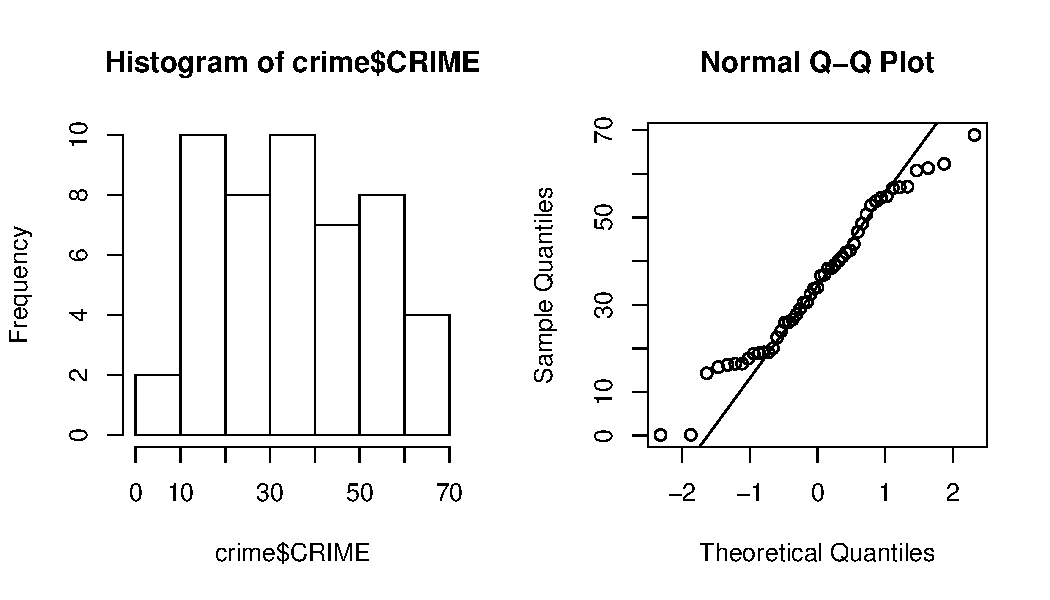
\includegraphics[width=\maxwidth]{figure/CRIMEdesc} 

\end{knitrout}
\caption{Histogram and qqplot for the CRIME variable showing departure from normality}
\label{crime}
\end{figure}

\begin{figure}
\begin{knitrout}
\definecolor{shadecolor}{rgb}{0.969, 0.969, 0.969}\color{fgcolor}\begin{kframe}
\begin{alltt}
\hlkwd{par}\hlstd{(}\hlkwc{mfrow}\hlstd{=}\hlkwd{c}\hlstd{(}\hlnum{1}\hlstd{,}\hlnum{2}\hlstd{))}
\hlkwd{hist}\hlstd{(crime}\hlopt{$}\hlstd{HOVAL,}\hlkwc{breaks}\hlstd{=}\hlstr{"Scott"}\hlstd{)}
\hlkwd{qqnorm}\hlstd{(crime}\hlopt{$}\hlstd{HOVAL)}
\hlkwd{qqline}\hlstd{(crime}\hlopt{$}\hlstd{HOVAL)}
\end{alltt}
\end{kframe}
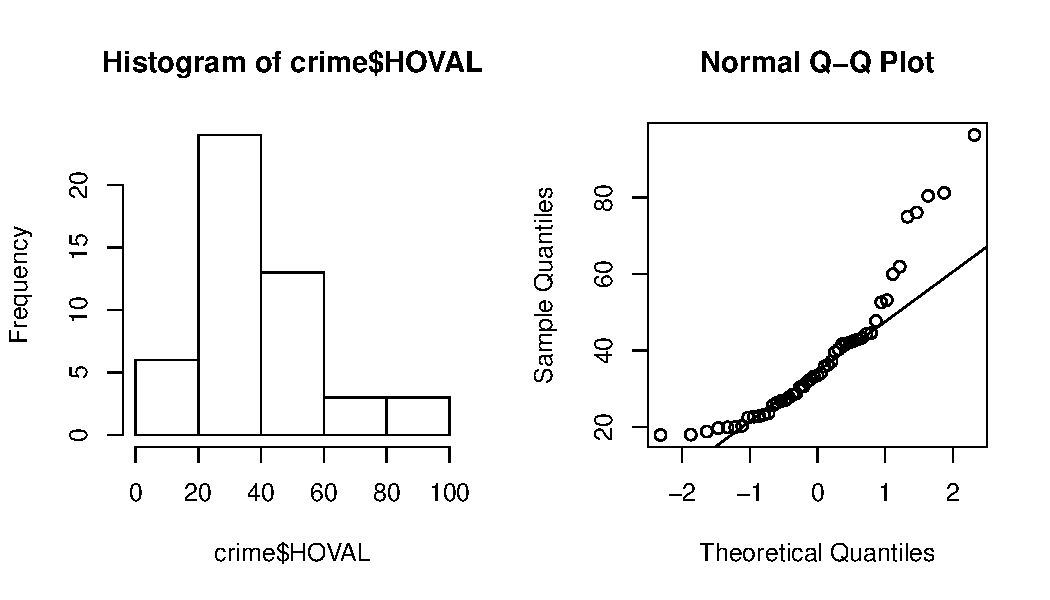
\includegraphics[width=\maxwidth]{figure/HOVALdes} 

\end{knitrout}
\caption{Histogram and qqplot for the variable ``HOVAL" showing severe depature from normality with a strong right skew.}
\label{hoval}
\end{figure}

\begin{figure}
\begin{knitrout}
\definecolor{shadecolor}{rgb}{0.969, 0.969, 0.969}\color{fgcolor}\begin{kframe}
\begin{alltt}
\hlkwd{par}\hlstd{(}\hlkwc{mfrow}\hlstd{=}\hlkwd{c}\hlstd{(}\hlnum{1}\hlstd{,}\hlnum{2}\hlstd{))}
\hlkwd{hist}\hlstd{(crime}\hlopt{$}\hlstd{INC,}\hlkwc{breaks}\hlstd{=}\hlstr{"Scott"}\hlstd{)}
\hlkwd{qqnorm}\hlstd{(crime}\hlopt{$}\hlstd{INC)}
\hlkwd{qqline}\hlstd{(crime}\hlopt{$}\hlstd{INC)}
\end{alltt}
\end{kframe}
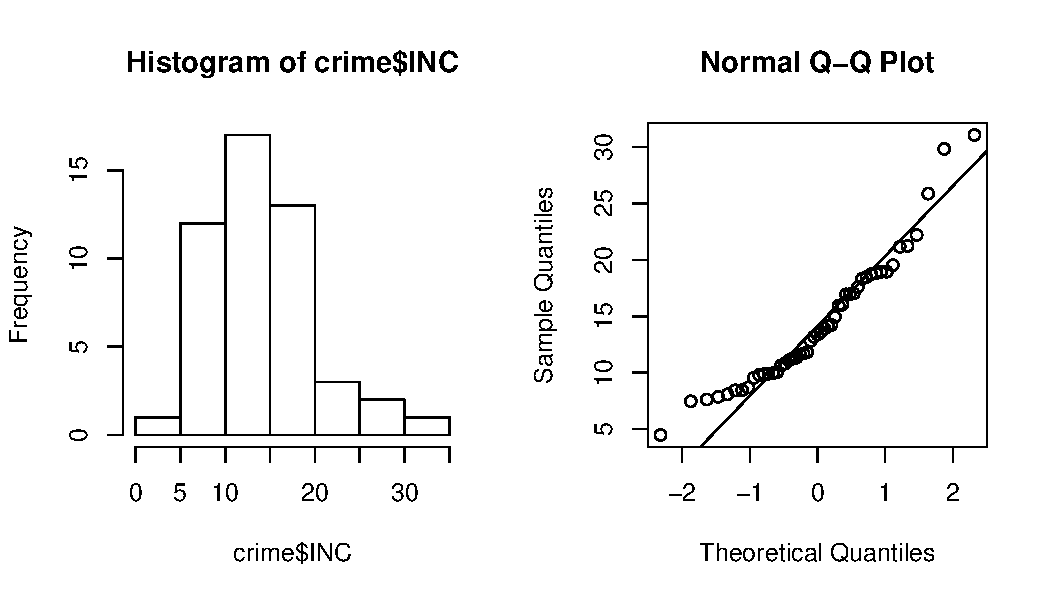
\includegraphics[width=\maxwidth]{figure/INCdesc} 
\begin{kframe}\begin{alltt}
\hlkwd{par}\hlstd{(}\hlkwc{mfrow}\hlstd{=}\hlkwd{c}\hlstd{(}\hlnum{1}\hlstd{,}\hlnum{1}\hlstd{))}
\end{alltt}
\end{kframe}
\end{knitrout}
\caption{Histogram and qqplot for the variable ``INC" showing the strong right skew and departure from normality}
\label{inc}
\end{figure}
\FloatBarrier

To see the relationship between these variables we can look at a scatterplot matrix (figure~\ref{scatmat}). We can see from this matrix that the income is positively correlated with home value and both home value and income are negatively correlated with crime.\\

\begin{figure}[hb]
\begin{knitrout}
\definecolor{shadecolor}{rgb}{0.969, 0.969, 0.969}\color{fgcolor}\begin{kframe}
\begin{alltt}
\hlkwd{plot}\hlstd{(crime[,}\hlkwd{c}\hlstd{(}\hlstr{"INC"}\hlstd{,}\hlstr{"HOVAL"}\hlstd{,}\hlstr{"CRIME"}\hlstd{)])}
\end{alltt}
\end{kframe}
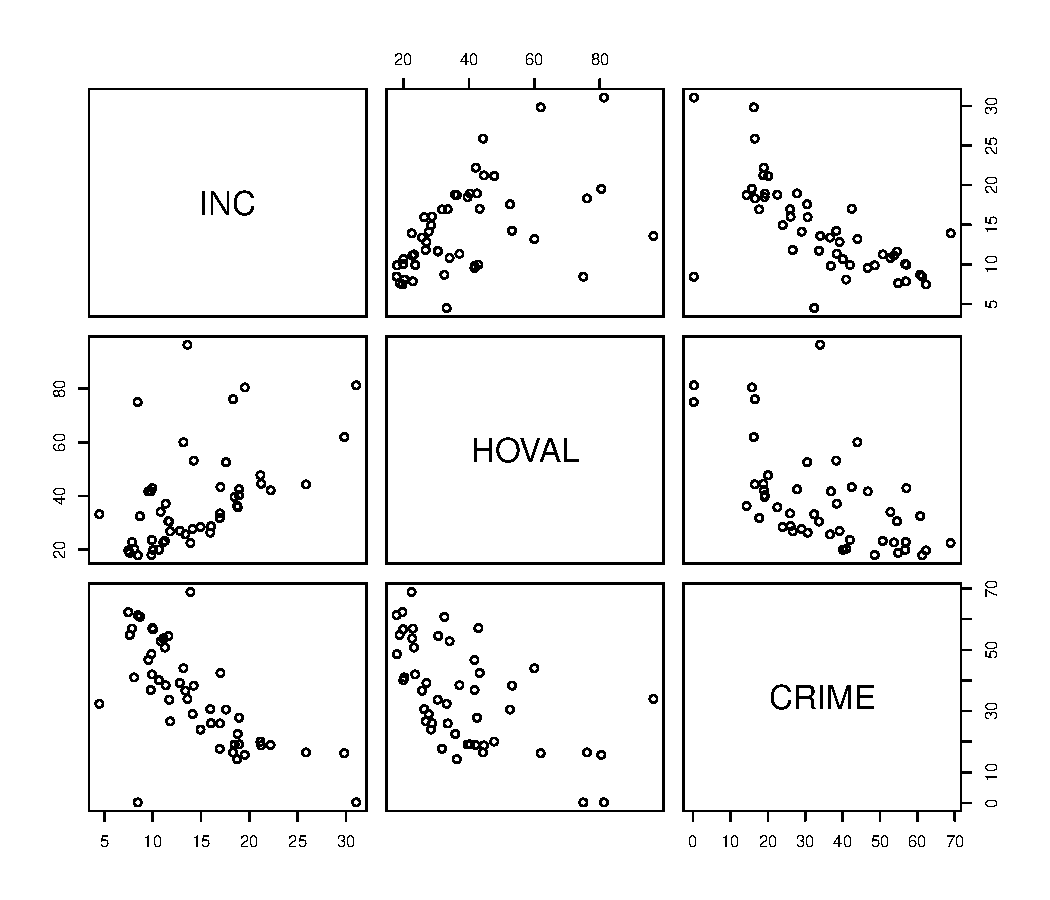
\includegraphics[width=\maxwidth]{figure/scatmat} 

\end{knitrout}
\caption{Scatterplot matrix of variables ``INC", ``HOVAL", and ``CRIME" showing a positive relationship between ``INC" and ``HOVAL" and negative relationships between ``INC" and ``CRIME" as well as ``CRIME" and ``HOVAL".}
\label{scatmat}
\end{figure}

\begin{knitrout}
\definecolor{shadecolor}{rgb}{0.969, 0.969, 0.969}\color{fgcolor}\begin{kframe}
\begin{alltt}
\hlstd{m1}\hlkwb{<-}\hlkwd{lm}\hlstd{(CRIME}\hlopt{~}\hlstd{INC}\hlopt{+}\hlstd{HOVAL,}\hlkwc{data}\hlstd{=crime)}
\hlstd{r1}\hlkwb{<-}\hlkwd{residuals}\hlstd{(m1)}
\hlstd{f1}\hlkwb{<-}\hlkwd{fitted}\hlstd{(m1)}
\end{alltt}
\end{kframe}
\end{knitrout}
We can model crime as a function of home value and income and get the following fitted model using maximum likelihood methods (equivalent to least-squares in this case).
$$CRIME = 68.619 + \ensuremath{-1.5973} \times INC + \ensuremath{-0.2739} \times HOVAL + \epsilon$$
We must check to see if the fitted model violates the normality assumption of the linear regression, i.e. that the residuals ($\epsilon$) are normally distributed.\\

\begin{figure}
\begin{knitrout}
\definecolor{shadecolor}{rgb}{0.969, 0.969, 0.969}\color{fgcolor}\begin{kframe}
\begin{alltt}
\hlkwd{par}\hlstd{(}\hlkwc{mfrow}\hlstd{=}\hlkwd{c}\hlstd{(}\hlnum{2}\hlstd{,}\hlnum{2}\hlstd{))}
\hlkwd{plot}\hlstd{(crime}\hlopt{$}\hlstd{CRIME}\hlopt{~}\hlstd{f1,} \hlkwc{ylab}\hlstd{=}\hlstr{"Crime"}\hlstd{,} \hlkwc{xlab}\hlstd{=}\hlstr{"Predicted Crime"}\hlstd{)}
\hlkwd{abline}\hlstd{(}\hlnum{0}\hlstd{,}\hlnum{1}\hlstd{)}
\hlkwd{plot}\hlstd{(crime}\hlopt{$}\hlstd{CRIME, r1,} \hlkwc{ylab}\hlstd{=}\hlstr{"Residuals"}\hlstd{)}
\hlkwd{abline}\hlstd{(}\hlkwc{h}\hlstd{=}\hlnum{0}\hlstd{)}
\hlkwd{hist}\hlstd{(r1,} \hlkwc{xlab}\hlstd{=}\hlstr{"Residuals"}\hlstd{)}
\hlkwd{qqnorm}\hlstd{(r1,} \hlkwc{ylab}\hlstd{=}\hlstr{"Residuals"}\hlstd{)}
\hlkwd{qqline}\hlstd{(r1)}
\end{alltt}
\end{kframe}
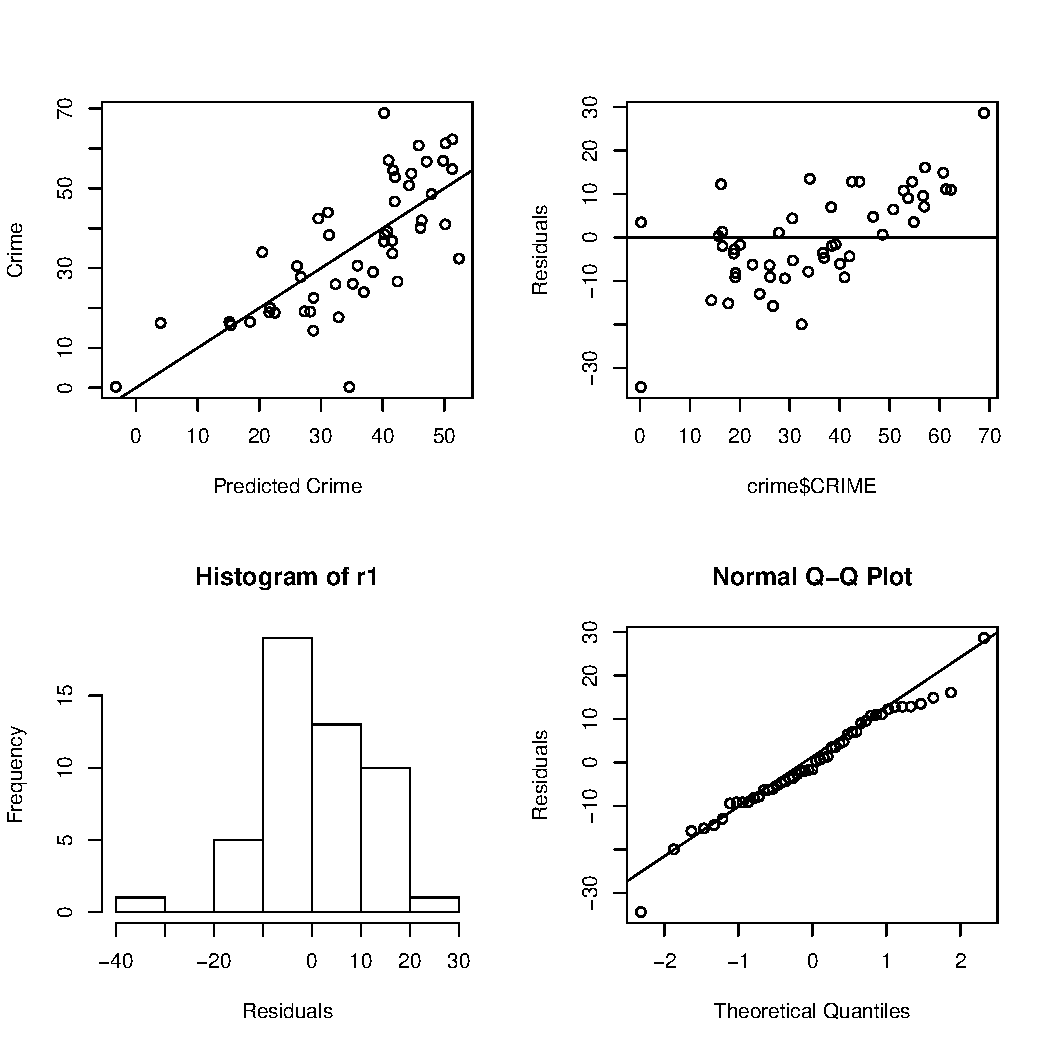
\includegraphics[width=\maxwidth]{figure/checkresid} 
\begin{kframe}\begin{alltt}
\hlkwd{par}\hlstd{(}\hlkwc{mfrow}\hlstd{=}\hlkwd{c}\hlstd{(}\hlnum{1}\hlstd{,}\hlnum{1}\hlstd{))}
\end{alltt}
\end{kframe}
\end{knitrout}
\caption{Inspection of predicted vs observed values as well as the residuals indicates that the normality assumption generally holds for this model}
\label{check}
\end{figure}

\end{document}
